\asection{Data Set}
\label{Data Set}

The graph data that is used in the experimentation was created by David S. Johnson, Cecilia R. Aragon,Lyle A. McGeoch and Catherine Schevon [14]. 
It was created in 1991 to study optimization by simulated annealing. One of the graphs that used was chosen to be experimented on to study the subject
algorithms, namely the Ullman and VF2 algorithms. The graph used can be found here [14].\newline\newline
The graph is a large direct graph that comprises of 250 vertices and 3218 edges [14], and it is used as the super-graph in the experiments, 
and will be refered to as the subject-graph from here on out. Figure ~\ref{fig:250} depicts a diagram of how the graph looks like.\newline\newline
The algorithms both need two graph in order to determine if they are isomorphically related to each other or not, thus subgraphs from our object graph
are required for this comparison. These subgraphs are then generated from the object graph and they all meet the condition that:
\begin{itemize}
  \item They are either partially or completely isomorphic in relation to one or other digraph inside the set.
\end{itemize}

\begin{figure}[H]
  \begin{center}
      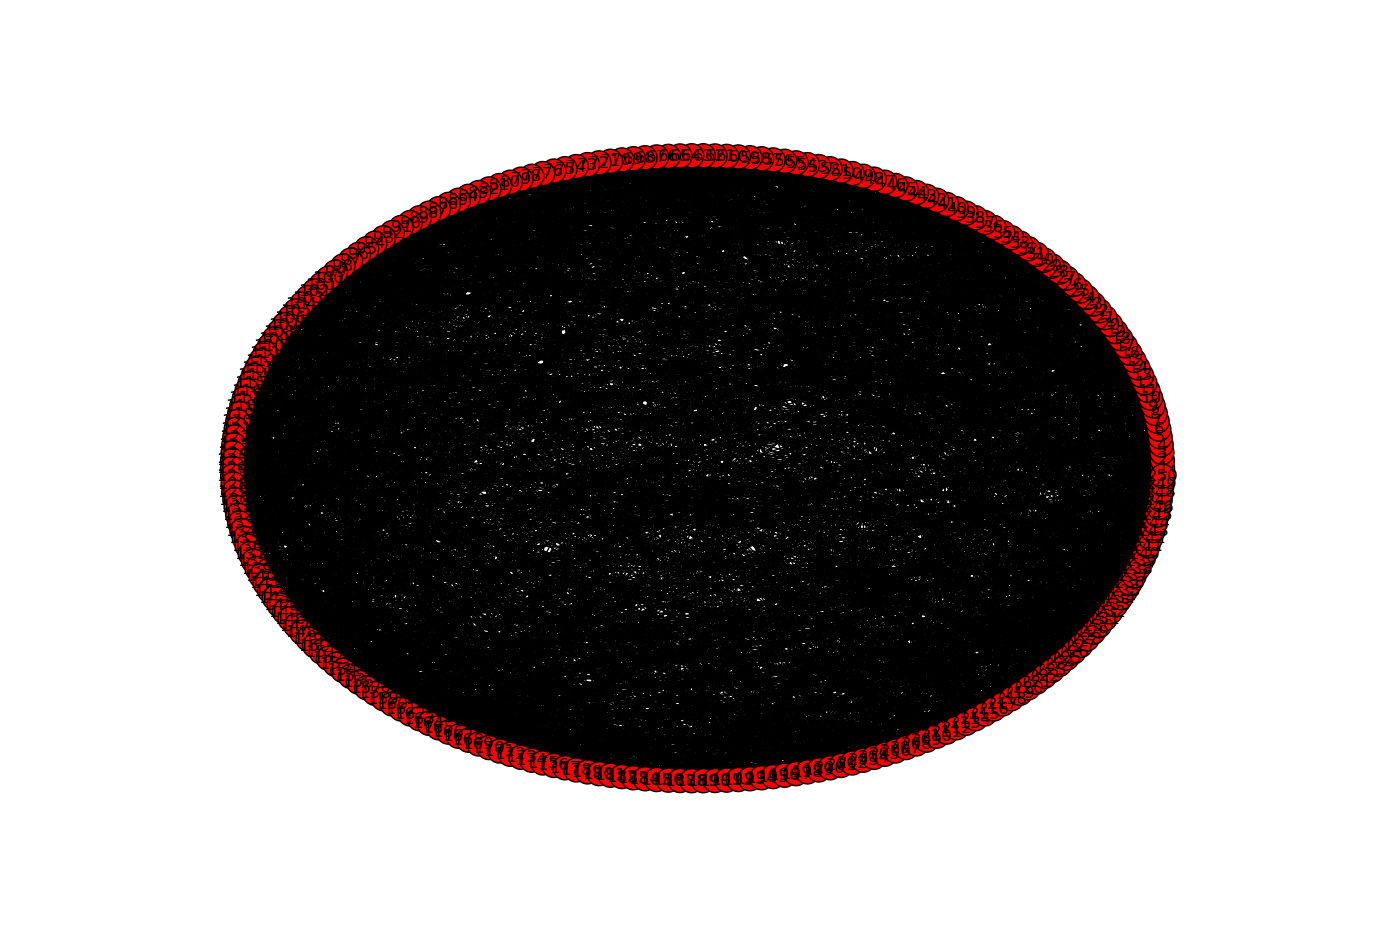
\includegraphics[width=1.0\textwidth]{250.png}
  \end{center}    
  \caption{The super-graph used in the experiment comprising of 250 vertices}
  \label{fig:250}
\end{figure} 
The subgraphs will be refered to as subject-graphs from here on out.\newline\newline
The generated subgraphs have the following number of vertices: 30,56,75,92,109,121,148,166,181,197,211 and 222. Each one of the graphs is sub-graph isomorphic to
the object graph, and will compared with it to determine how long it takes to find the isomorphic relationship, and how much virtual memory [15] is used to find 
the relationship.\newline
Figure ~\ref{fig:generatedSubs} depics how some of the generated subgraphs lot relative to figure Figure ~\ref{fig:250}.

\begin{figure}[!htbp]

  \begin{subfigure}[b]{0.6\textwidth}
    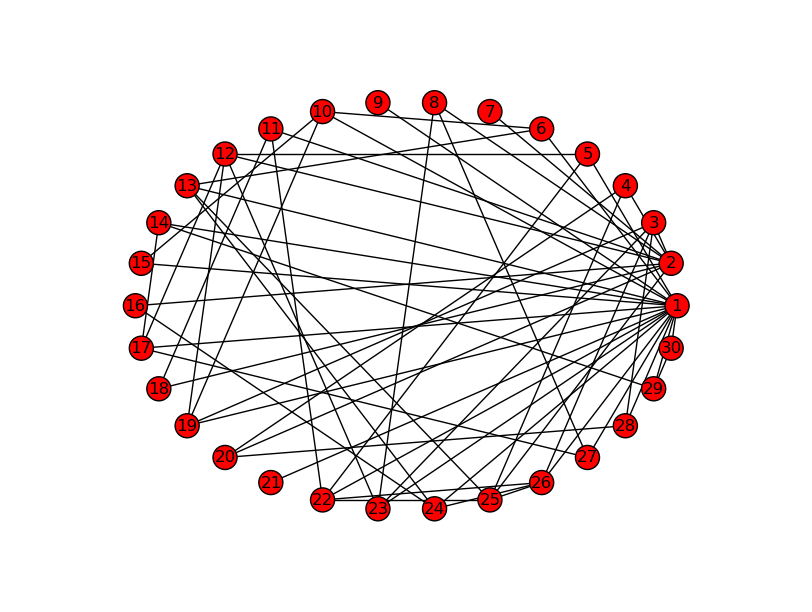
\includegraphics[width=\textwidth]{30}
    \caption{Generated subgraph with 30 vertices}
    \label{fig:30}
  \end{subfigure}
  \hfill
  \begin{subfigure}[b]{0.6\textwidth}
    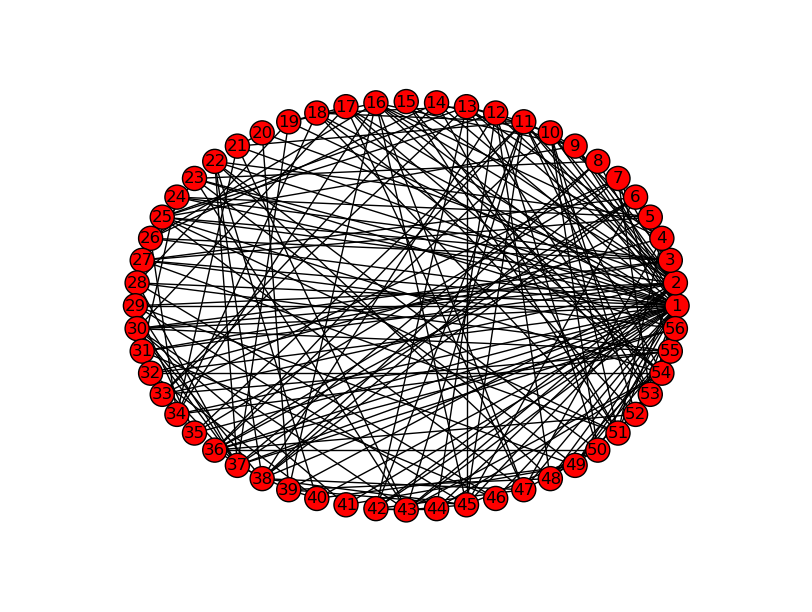
\includegraphics[width=\textwidth]{56}
    \caption{Generated subgraph with 56 vertices}
    \label{fig:56}
  \end{subfigure}
  \begin{subfigure}[b]{0.6\textwidth}
    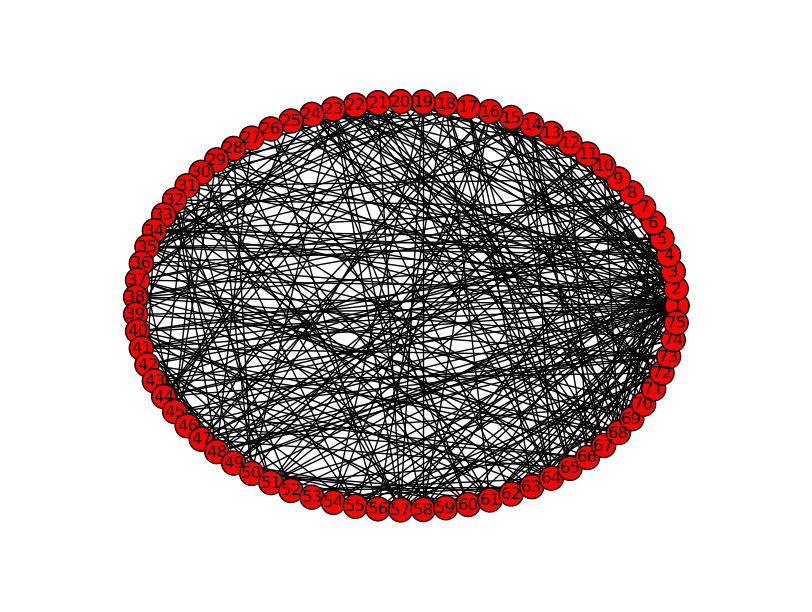
\includegraphics[width=\textwidth]{75}
    \caption{Generated subgraph with 75 vertices}
    \label{fig:75}
  \end{subfigure}
  \hfill
  \begin{subfigure}[b]{0.6\textwidth}
    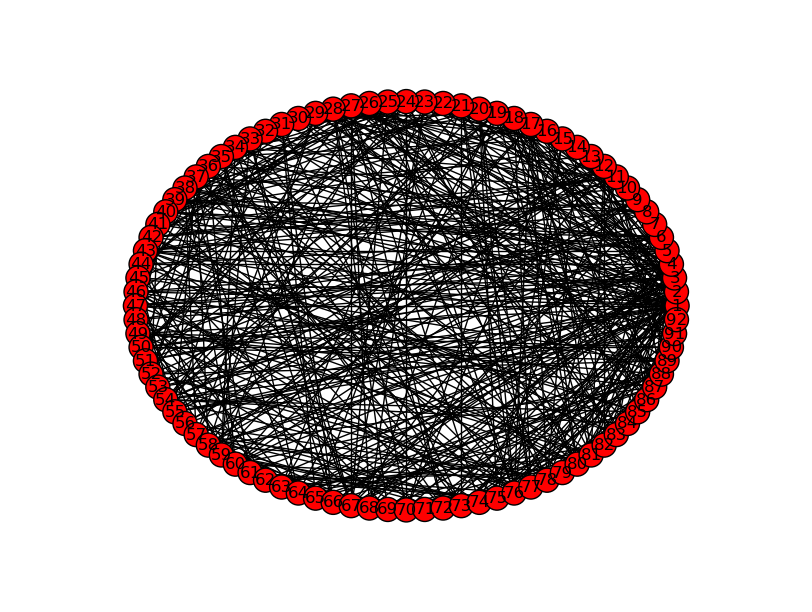
\includegraphics[width=\textwidth]{92}
    \caption{Generated subgraph with 92 vertices}
    \label{fig:92}
  \end{subfigure}
  \begin{subfigure}[b]{0.6\textwidth}
    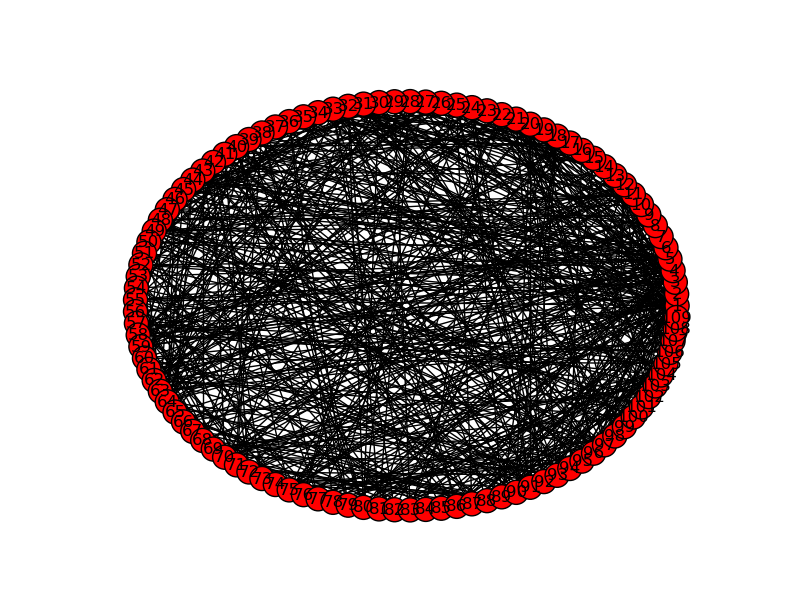
\includegraphics[width=\textwidth]{109}
    \caption{Generated subgraph with 109 vertices}
    \label{fig:109}
  \end{subfigure}
  \hfill
  \begin{subfigure}[b]{0.6\textwidth}
    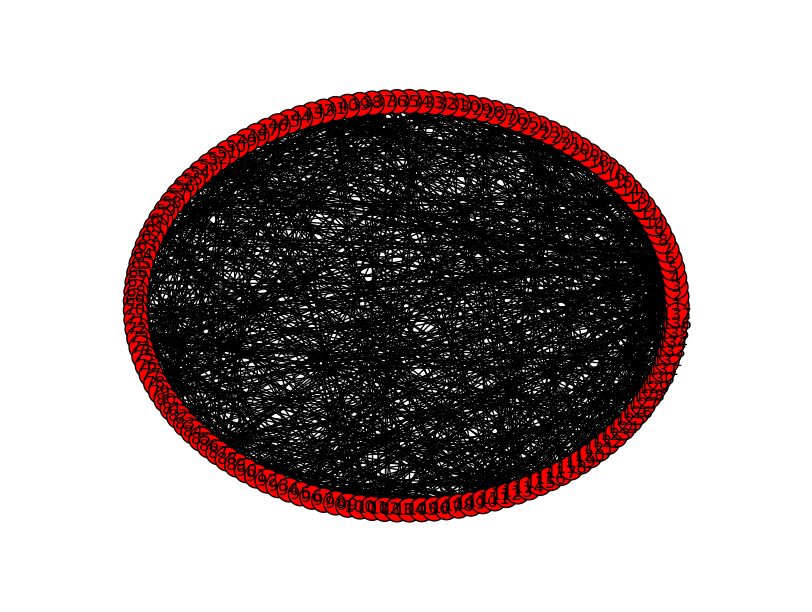
\includegraphics[width=\textwidth]{121}
    \caption{Generated subgraph with 121 vertices}
    \label{fig:121}
  \end{subfigure}
  \caption{A demostration of two isomorphic graphs}
  \label{fig:generatedSubs}  
\end{figure}

\newpage